\chapter{Augmented Reality}

Im Gegensatz zu \glqq Virtual Reality\grqq{} (VR), welche eine interaktive, dreidimensionale, computergenerierte, immersive Umgebung schafft, in die eine Person versetzt wird, erlaubt \glqq Augmented Reality\grqq{} (AR) die Überblendung von digitalen Medieninformationen über die Wahrnehmung der echten Welt. Dadurch fällt AR in die Definition von \glqq Mixed Reality\grqq{} (MR).

\begin{figure}[H]
	\centering
	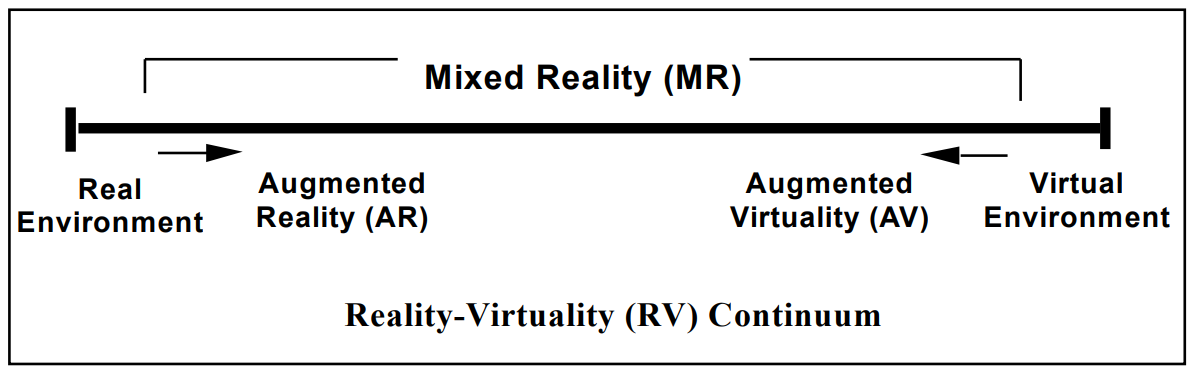
\includegraphics[scale=0.52]{ar_vr.png}
	\caption{Das Realität - Virtualität Kontinuum, Bildquelle \cite{ar_vr}}
\end{figure} 

Im Rahmen dieser Arbeit wird sich, wenn der Begriff Augmented Reality verwendet wird, auf Monitor basierte, nicht immersive Geräte bezogen, da bei der Analyse von Photogrammetrie und Computer Vision sowie der Implementation einer AR Anwendung, das Smartphone als Medium im Fokus steht. Diese Anzeigesysteme werden auch als \glqq window-on-the-world\grqq{} bezeichnet, da computergenerierte Bilder oder Informationen digital über das wiedergegebene Echtzeit Kamera Bild des Smartphones überlagert werden. (vgl. \cite{ar_vr} S.284)



\section{Augmented Reality - SDKs}

\glqq Software Development Kits\grqq{} (SDK) oder auch Frameworks, sind Werkzeuge und Bibliotheken, welche Algorithmen und Basistechnologien liefern, um Programme zu entwickeln. Im Bereich von Augmented Reality umfassen Frameworks meistens die drei Hauptkomponenten (vgl. \cite{sdks} S.3):

\begin{itemize}

\item \textbf{Recognition}: Erkennung von Bildern, Objekten, Gesichtern oder Räumen, auf welche die virtuellen Objekte oder Informationen überlagert werden können.


\item \textbf{Tracking}: Echtzeit-Lokalisierung der erkannten Objekte und Berechnung der lokalen Position des Gerätes zu diesen.

\item \textbf{Rendering}: Überlagerung der virtuellen Medieninformationen über das Bild und Anzeige der generieren Mixed Reality.
\end{itemize}

\subsection{Marktübersicht - Software Development Kits}

Die folgende Tabelle gibt eine Übersicht an aktuellen und weit verbreiteten Software Development Kits, sowie deren Plattformkompatibilität zu Android und iOS: \\

\begin{table}[h!]
\hskip-1.5cm
\begin{tabular}{|l|l|l|l|l|l|l|l|l|l|}
\hline
        & Vuforia & Wikitude & Metaio & ARToolKit & Kudan & EasyAR & MaxST & ARCore & ARKit \\ \hline
Android &   \checkmark      &    \checkmark      &    \checkmark    &     \checkmark      &   \checkmark    &    \checkmark    &    \checkmark   &     \checkmark   &    x   \\ \hline
iOS     &    \checkmark      &   \checkmark        &   \checkmark      &    \checkmark        &   \checkmark    &    \checkmark     &   \checkmark     &    \checkmark     &    \checkmark    \\ \hline
Windows &     \checkmark     &    \checkmark       &     \checkmark    &    \checkmark        &   x    &     \checkmark    &  \checkmark      &    x    &    x   \\ \hline
\end{tabular}
\end{table} 


Bis auf das von Apple entwickelte ARKit, sind alle hier genannten Frameworks für Android verwendbar. Weiterhin unterstützen alle das Betriebsystem iOS, sowie Windows, bis auf Kudan, ARCore und ARKit. Im praktischen Teil dieser Arbeit werden mehrere dieser Software Development Kits auf der Android Plattform verwendet, getestet und analysiert.

\section{Voraussetzungen für Augmented Reality}
Augmented Reality Anwendungen haben hohe Anforderungen an die Rechnenpower der Technik, die Verarbeitungsgeschwindigkeit der Algorithmen und Robustheit der verwendeten Verfahren. Folgende Liste gibt eine Übersicht an wichtigen Aspekten um AR zu realisieren  (vgl. \cite{vorraussetzungen} S.1):


\begin{itemize}

\item \textbf{Hohe räumliche Genauigkeit}: 6 \glqq Degrees of Freedom\grqq{} (Freiheitsgrade) in Position und Ausrichtung. 

\item \textbf{Sehr geringer Jitter (Zittern)}: Das Rauschen im Tracking System muss minimal gehalten werden.

\item \textbf{Hohe Aktualisierungsraten}: mindestens 30Hz, besser mehrere 100Hz.

\item \textbf{Sehr geringer Lag}: Die Verzögerung von Messung bis zur Trackerausgabe muss minimal sein.

\item \textbf{Volle Mobilität}: Bewegungsfreiheit für den Nutzer: Keine Kabel, kein eingeschränkte Umfang an Bedienmöglichkeiten.
\end{itemize}

Erst durch die Entwicklung der Technik in den letzten zwei Jahrzehnten und einer damit eingehenden Steigerung der Rechenpower von mobilen Geräten, hat sich Augmented Reality auf Smartphones etablieren können.

\section{Arten des Augmented Reality Trackings}

Das Erkennen der Umgebung und die Lokalisierung der Kamera (Camera Pose Estimation) in dieser, siehe Abbildung 2.2, ist der ausschlaggebende Schritt zur Realisierung von Augmented Reality. Erst dieses Verfahren erlaubt die Projektion von digitalen Modellen in der richtigen Position auf den echten Bildern, um die Perspektiven von echter Welt und digitalem Modell zu vereinen. 


\begin{figure}[H]
	\centering
	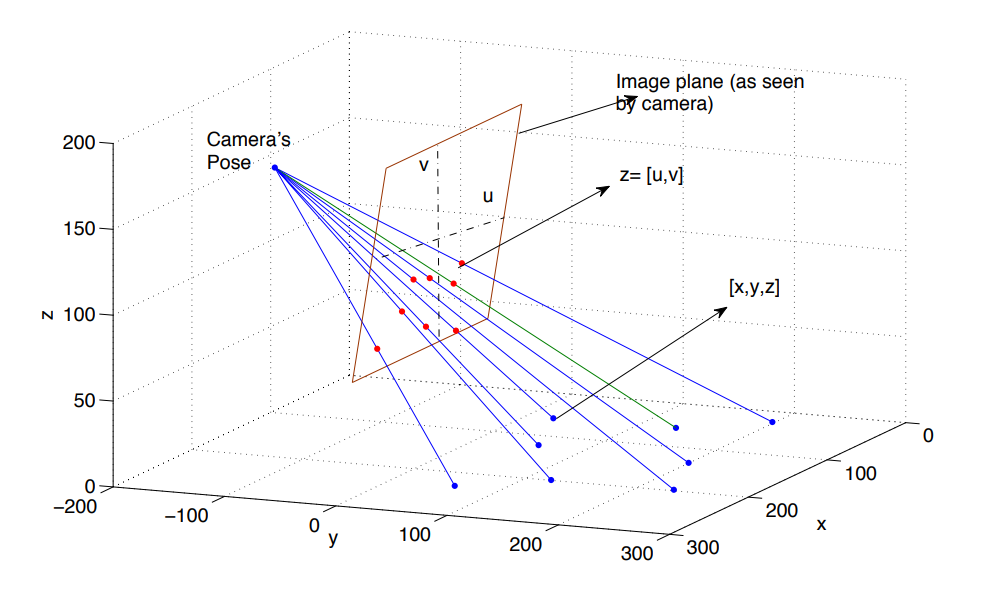
\includegraphics[scale=0.58]{pose.png}
	\caption{Kamera Posenschätzung, anhand von Markern. Bildquelle \cite{pose}}
\end{figure} 


Präzise und robuste Kamerapositionsdaten sind eine Grundvoraussetzung für eine Vielzahl von Anwendungen, wie dynamischer Szenenanalyse und Interpretation, 3D-Szenen Strukturerkennung oder Videodatenkompression. Augmented Reality Umgebungen sind ein komplexes Anwendungsgebiet der Kameralokalisierung, da ein eingeschränkter Arbeitsbereich, limitierte Rechenpower und spezifische Anwendungsfälle hohe Anforderungen an die Robustheit und Schnelligkeit der Algorithmen stellen. 
Es existieren viele verschiedene Ansätze, um die Kameralokalisierung im Raum zu lösen. Das Problem wird als nichtlineares Problem betrachtet und wird meistens durch die \glqq Method of Least Squares\grqq{} (Methode der kleinsten Quadrate) oder  mit nichtlinearen Optimierungsalgorithmen gelöst, typischerweise durch das Gauß-Newton oder Levenberg-Marquardt Verfahren. (vgl. \cite{camera_pose} S.1) Im Folgenden werden die vier gängigsten Ansätze zur Lösung des Tracking Problems erläutert. 


\subsection{Referenzmarken-basiertes Tracking}

Markerbasiertes Tracking war lange Zeit eine der häufigsten verwendeten Techniken um Augmented Realtiy zu realisieren. Dies liegt in der einfachen Erkennung der Marker mit hohem Kontrast.

\begin{figure}[H]
	\centering
	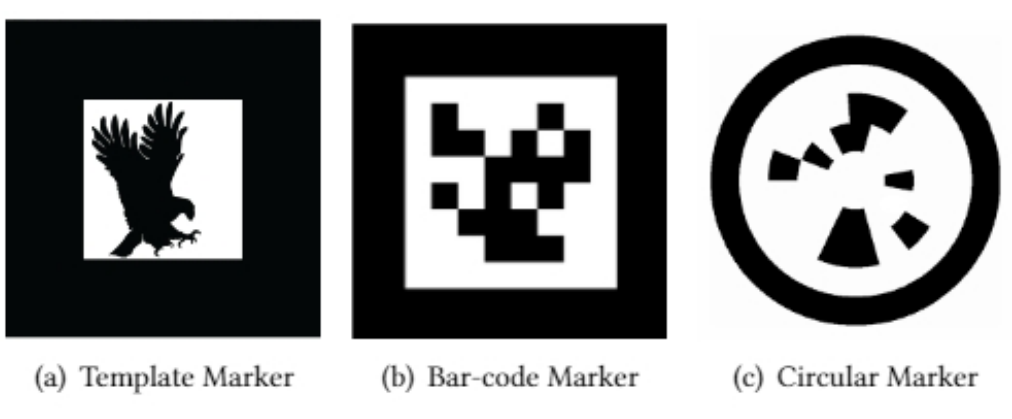
\includegraphics[scale=0.6]{markers.png}
	\caption{Moderne Marker. Bildquelle \cite{markers}}
\end{figure} 

Für robuste Anwendungen werden meist schwarz-weiße Marker mit dicken Kanten verwendet, siehe Abbildung 2.3. Die Kanten dienen der Erkennung des Markers, das einzigartige Muster zur genauen Identifizierung, um welchen einzigartigen Marker es sich handelt (vgl. \cite{markers} S.2). Dadurch kann neben der Relation des Geräts zum Marker auch relativ einfach die Entfernung und der Winkel berechnet werden. Der Nachteil liegt in der Limitierung der Anwendungsgebiete, in denen diese Technik verwendet werden kann, da Marker immer im Sichtfeld der Kamera lokalisiert sein müssen und nicht von anderen Objekten verdeckt werden dürfen. Weiterhin müssen immer externe Ressourcen verwendet werden um diese Marker zu erstellen, zu registrieren und zu verwenden, was bei der Verwendung der Anwendung und damit der Nutzerfreundlicheit, immer mit einem Mehraufwand verbunden ist (vgl. \cite{comparative_sdks} S.13).

\subsection{Hybrid-basiertes Tracking}

Hybrid basiertes Tracking verwendet mehrere Datenquellen wie das Global Positioning System (GPS), den Kompass oder die Beschleunigungssensoren des Smartphones zur Bestimmung der Orientierung und Lokalisierung des Geräts. Dabei wird per GPS der Standort des Geräts bestimmt, um Objekte in der Nähe zu identifizieren, die augmentiert werden sollen. Mit Hilfe des Kompasses kann dann ein Pfad erstellt und überprüft werden, ob die Orientierung des Geräts auch in diese Richtung zeigt. Der Beschleunigungssensor bestimmt die Ausrichtung des Geräts mithilfe der Gravitation. Durch die Vereinigung all dieser Informationen aus den Sensoren, kann berechnet werden, was im Sichtfeld ergänzt werden soll, ohne dass eine Auswertung und Verarbeitung des realen aufgenommen zweidimensionalen Kamerabildes stattzufinden hat. Anschließend werden die Informationen über das Kamerabild gelegt.  (vgl. \cite{comparative_sdks} S.13, \cite{vorraussetzungen} S.4)

\subsection{Modell-basiertes Tracking}

Beim Modell-basiertem Tracking wird ein rekursiver Algorithmus verwendet. Hierbei wird die vorherige Kameraposition als Grundlage für die Berechnung der aktuellen Kameraposition verwendet. Dazu muss zuerst eine Kamerakalibrierung durchgeführt werden, anschließend wird die Pose des zu verfolgenden Objekts initial bestimmt. Dann wird bestimmt, welche Ecken des Objekts sichtbar sind. An diesen Ecken werden dann Kontrollpunkte verteilt, die in späteren rekursiven Aufrufen mit denen älterer Frames verglichen werden, was mit einer Karte der Ecken ermöglicht wird. Die Map der Ecken wird mithilfe des Canny-Algorithmus zur Eckenerkennung erstellt. Ist die Abweichung zum vorherigen Frame bestimmt worden, wird die Position der Kamera im Bezug zum Objekt aktualisiert. Durch die Rekursivität ist dieses Verfahren nicht sehr rechenintensiv und benötigt eine relativ geringe Prozessorleistung. Weiterhin kann zwischen verschiedenen Merkmalen unterschieden werden, welche für das Tracking verwendet werden. Bei der kantenbasierten Methode wird versucht ein dreidimensionales Wireframe mit den Kanten des Objekts in der realen Welt zuzuordnen. (vgl. \cite{model_based} S.2-3)

\begin{figure}[H]
	\centering
	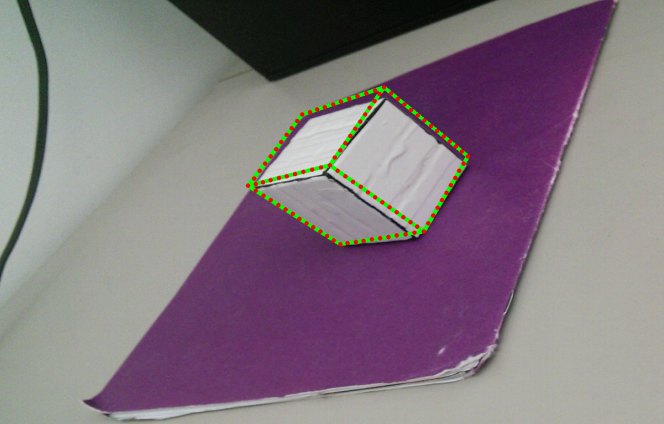
\includegraphics[scale=0.75]{wire.png}
	\caption{Kantenbasiertes rekursives Tracking, Pipeline. Bildquelle: \cite{model_based} S.3}
\end{figure} 

Außerdem sind Ansätze wie \glqq Optical Flow based Tracking\grqq{}, was zeitliche Informationen, entnommen aus der Bewegung der Projektion des Objekts relativ zur Bildebene verwendet, sowie texturbasierte Ansätze verbreitet. (vgl. \cite{model_based} S.1)

\subsection{Natürliches Feature Tracking}

Natürliches Feature Tracking ist ein bildbasiertes Verfahren und kann die Position des Gerätes zur Umgebung bestimmen, ohne über Wissen über einen initialen vorherigen Zustand zu verfügen. Diese Methode ist in der Regel sehr rechenintensiv und benötigt hohe Prozessorleistung (vgl. \cite{model_based} S.1-2). Die Technik verwendet die Merkmale von Objekten in der echten Welt und erkennt ihre natürlichen Eigenschaften. Diese Merkmale werden \glqq Features\grqq{} genannt und sind typischerweise, basierend auf einem mathematischem Algorithmus, sehr gut unterscheidbar und außern sich in der Form von Ecken, Kanten oder starke Kontrasten. Die mathematischen Beschreibungen dieser Features (Deskriptoren) eines Bildes werden zur späteren Erkennung gespeichert. Anhand des gespeicherten Datensets aus Merkmalen kann dann erkannt werden, ob ein Bild im Vergleich zu einem anderen den gleichen Inhalt zeigt, unabhängig von Entfernung, Orientierung, Beleuchtungsintensität, Rauschen oder Verdeckung (vgl. \cite{comparative_sdks} S.13). Beim natürlichen Feature Tracking wird, meistens basierend auf dem Verfahren der kleinsten Quadrate und mit dem Gauß-Newton oder Levenberg-Marquardt Verfahren, versucht eine Reduzierung des \glqq Re-Projection Errors\grqq{} (Reprojektionsfehlers) zu erreichen, um alle internen und externen Kameraparameter zu bestimmen und zu optimieren. Dies sind nicht-lineare Methoden zur Lösung des Problems der kleinsten Quadrate. Typischerweise sind zwei bis vier Wiederholungen genug. (vgl. \cite{natural_feature} S.28-29) Die genaue Funktionsweise des Natürlichen Feature Trackings wird in Kapitel 3.5 und 3.6 weiter ausgeführt.
 

\section{Photogrammetrie oder Computer Vision für AR}

In Kapitel 2 wurde eine kurze Einführung in Augmented Reality gegeben und deren Voraussetzungen sowie aktuellen Umsetzungen der Kameralokalisierung vorgestellt. Im folgenden Teil dieser Arbeit wird Photogrammetrie, sowie Verfahren aus der Computer Vision, wie etwa SLAM (Simultaneous Localisation and Mapping), welches von den meisten Augmented Reality Software Development Kits heutzutage verwendet wird, beschrieben. Weiterhin wird ein Vergleich der beiden Verfahren durchgeführt, um Gemeinsamkeiten, Unterschiede, sowie Möglichkeiten und Schwächen der einzelnen Verfahren aufzuzeigen und in Kontext zu bringen. Anschließend wird evaluiert ob photogrammetrische Verfahren in Kontext der Augmented Reality eingesetzt werden können.

